% Chapter 2
\chapter{RELATED WORK} % Chapter Title in ALL CAPSacs
This chapter gives a survey of the possible approaches for insurance management and other fields where blockchain can be leveraged. The section 2.1 discusses the existing approaches for insurance management.The section 2.2 discusses the implementation of Internet of Things in  insurance.  Blockchain technology has
gained significant importance due to its power for decentralizing techniques which previously worked in a centralized manner. Thus, researchers are trying to apply blockchain technology in different fields. The section 2.3 discusses about the utilization of blockchain technology in different fields. The section 2.4 discusses the financial applications of blockchain. The section 2.5 discusses the non-financial applications of blockchain. The section 2.6 discusses the implementation of blockchain in Internet Of Things.

\section{Artificial Intelligence}
\lipsum[]
Automation and AI have transformed almost every sector across the world, and the insurance industry is no exception. According to Accenture’s Technology Vision for Insurance 2017, 94 percent of “insurance executives agree that adopting a platform-based business model and engaging in ecosystems with digital partners are critical to their business.” In 2016, 35 percent of insurers reported over 15 percent in cost savings from automating systems and processes in the last two years. Automation of more complex tasks (other than compliance checks or data entry) such as property assessment and personalized consumer interactions over the years has brought frictionless experiences and cut down redundancy. 

Employing AI in the claims process has brought better quality and lesser time for handling. AI algorithms can save millions lost to fraudulent claims by scouring data and identify errors and trends. The future is definitely touchless. Machine learning can be useful in evaluating risk and identifying cross-selling opportunities. Online-only insurance technology companies, uses AI, machine learning, and big data to “simplify insurance, price risk more finely and distribute cheaply to a mass market via the internet.” For automated claims processing and property assessment, P&C insurance providers are using drones for more accurate information and faster processing.
\section{Internet of Things in Insurance}
\lipsum[]
IoT devices, sensors, and telematics have been fast gaining adoption in the insurance sector. Several data streams and sources (wearables, sensors embedded in vehicles, location-based sensors, GIS) coupled with advanced analytics can help insurers improve risk assessment, price policies based on real data in real time, and proactively encourage customers to buy policies for loss prevention. More usage-based insurance models for connected vehicles and precise actuarial models are expected with the huge amounts of data (or touchpoints) available thanks to today’s amazingly connected world. In the auto insurance sector, for example, the data (speed, time, braking patterns, distance) gives buyers more say in their premiums; risky driving patterns can serve as warning signs. Blockchain can be the “network connecting and ordering data from the multiple devices and apps involved in a multidimensional process.” (EY, 2016) It can help manage the huge volumes by ensuring P2P device communication.

Companies such as Aviva and State Farm urge customers to invest in home sensors (others such as FitSense deal with fit tech to help insurers), incentivizing them to help prevent risk to self (e.g. elderly care) and property. For example, Neos Ventures, UK’s first connected home insurance specialist, provides preventative smart technology as part of the policy.

Along with the real-time data and advanced digital capabilities, insurers enjoy better customer relationships and risk management, quicker processing of claims, and selling bundled products. Automating and streamlining so many data-driven insurance-related processes such as pricing policies, underwriting, approximating required reserves, and risk profiling help providers come up with valuable, easy-to-use, and affordable products and services.

\section{Blockchain}
\lipsum[]
In the cryptocurrency scenario, the issue between payer and payee is that there has to be a trusted third party to verify the double-spending of money and validate the transactions. It leads to a state where all the participating people has to agree on the trusted authority. The fate of the entire community is given to a single company that run the trusted authority. To make all participants of the network to agree upon transactions that were previously made it is important for all the participants to know all previous transactions. Thus a technology named blockchain is proposed to store all transactions in a public ledger in a tamper-resistant manner. 

A earlier cryptocurrency called bitcoin used a hard to solve Proof of Work to validate the transactions. Number of transactions bundled in a block is hashed in such a way that the hash contains some leading zeros. The computational complexity increases when number of leading zeros increases. Thus the whole network is given a CPU based voting permission. If the network contains more honest nodes controlling larger CPU power, then the network will have trusted larger chain of blocks.
\begin{figure}[htb!]
  \centering
 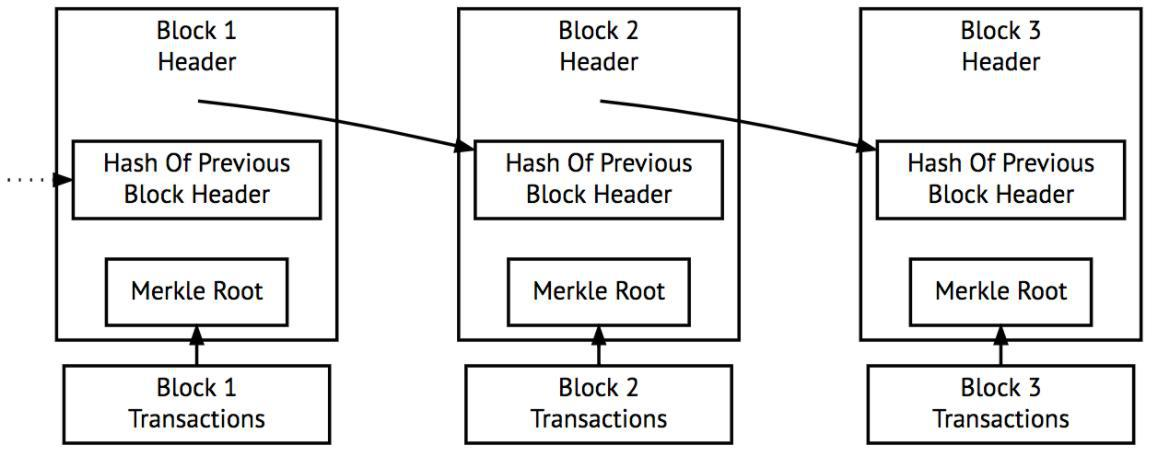
\includegraphics[width = 15cm, height = 6cm] {Figures/bitcoin.jpg}
  \caption{Blockchain in Bitcoin}
  \label{StH}	
\end{figure}
\newline

\section{Financial Applications of Blockchain}
\subsection{Stock Exchange}
The stock exchanges list company shares for secondary market to function securely with trades settling and clearing in a timely manner. It is now theoretically possible for companies to directly issue the shares via the blockchain. These shares can then be purchased and sold in a secondary market that sits on top of the blockchain. NASDAQ Private Equity has joined hands with a San Francisco based start-up to implement private equity exchange on top of blockchain.

\subsection{Assest Management}
Assets which can be uniquely identified by one or more identifiers that are difficult to destroy or replicate can be registered in blockchain. This can be used to verify ownership of an asset and also trace the transaction history. Any property (physical or digital such as real estate, automobiles, physical assets, laptops, other valuables) can potentially be registered in blockchain and the ownership, transaction history can be validated by anyone, especially insurers. Everledger is a company which creates permanent ledger of diamond certification and the transaction history of the diamond using blockchain. The verification of diamonds can be done by insurance companies, law enforcement agencies, owners and claimants easily using this blockchain.

\section{Non-Financial Applications of Blockchain}
\subsection{Health Care}
Estonia is implementing a blockchain based health care management record to store it in a hacker-proof manner. In that project, logs of access of health care data and audit data is stored in blockchain. All the users can see when the data is accessed but access log cannot be modified.

\subsection{Music Industry}
The process by which music royalties are determined has always been a convoluted one, but the emergence of the internet has made it even more complex giving rise to the demand of transparency in the royalty payments by both artists and song writers. This is where the blockchain can play a role. The technology can help maintain a comprehensive and accurate distributed database of music rights ownership information in a public ledger. In addition to rights ownership information, the royalty split for each work can be determined by smart contracts.

\subsection{Keyless Security Infrastructure}
Namecoin is an alternative blockchain technology that is used to implement a decentralized version of Domain Name Server. Current DNS servers are controlled by governments and large corporations, and could abuse their power to censor, hijack, or spy on a consumer’s internet usage. With blockchain technology internet’s DNS is maintained in a decentralized manner. Public Key Infrastructure technology is widely used for centralized distribution and management of digital certificates. Every device needs to have root certificate of the Certificate Authority to verify digital signature. While PKI has been widely deployed and incredibly successful, dependence on a CA makes scalability an issue. The characteristics of the blockchain can help address some of the limitations of the PKI by using Keyless Security Infrastructure.

\section{Blockchain in IoT}
Blockchain-IoT combination can work perfectly. For once us cases can be derived as follows.
\begin{enumerate}
  \item Facilitates the sharing of services and resources leading to the creation of a marketplace of services between devices.
  \item Allows us to automate in a cryptographically verifiable manner several existing, time-consuming workflows.
\end{enumerate}
There are some practical deployment difficulties in deploying IoT blockchain. These difficulties range from transactional privacy to the expected value of the digitized assets traded on the network.

Blockchain-IoT combination can be powerful and can cause significant transformations across several industries, paving the way for new business models, novel and distributed application, yet this blockchain model has some restrictions like scalability. The authors have talked about minimizing the data copied in a blockchain. They claim that security is not compromised using 51 percent attack yet minimizing the total data copied among the nodes. A new model of blockchain is proposed for limited memory availability using B language.
\begin{figure}[ht]
  \centering
 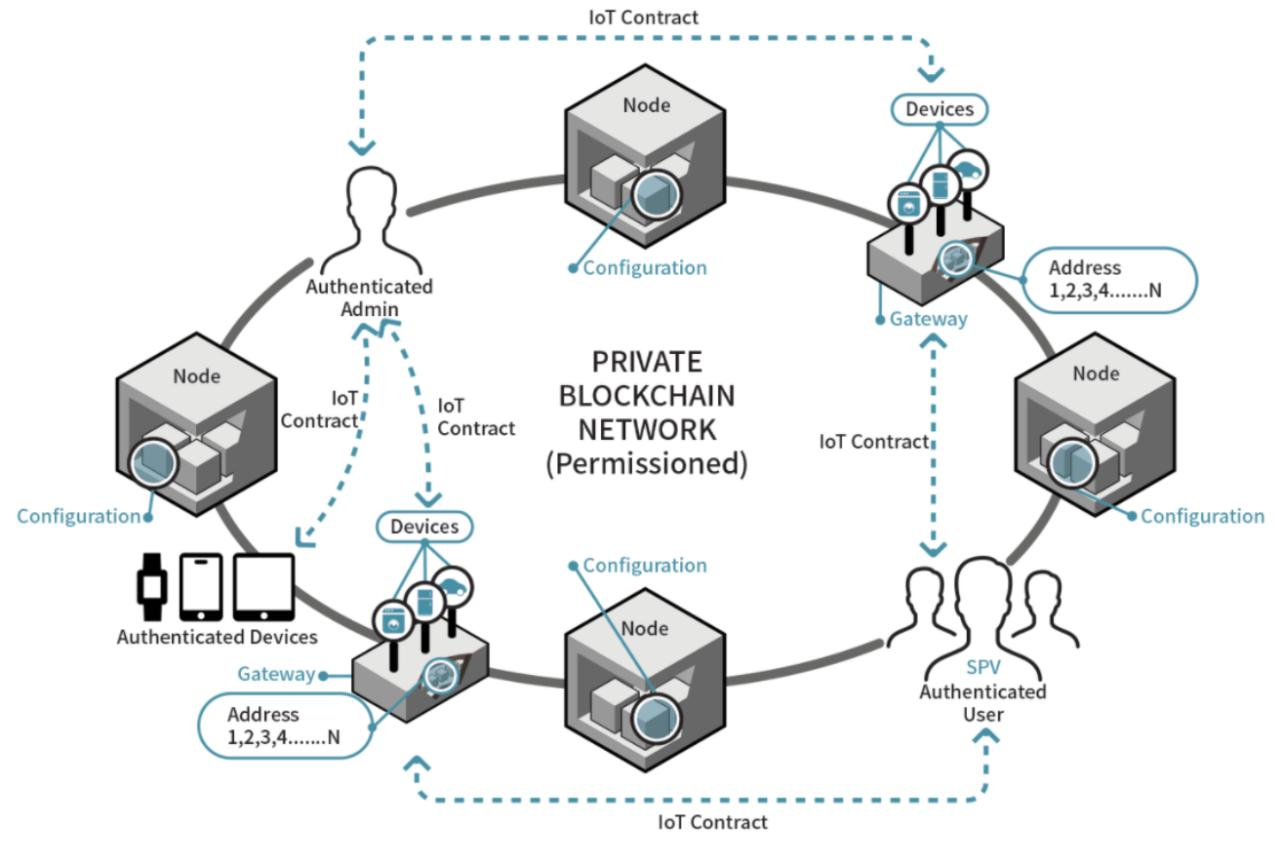
\includegraphics[width = 13cm, height = 8cm] {Figures/iot.jpg}
  \caption{Structure of Blockchain-IoT Network}
  \label{StH}	
\end{figure}
